% Diese Datei ist Teil des Buchs "Schreibe Dein Programm!"
% Das Buch ist lizensiert unter der Creative-Commons-Lizenz
% "Namensnennung - Weitergabe unter gleichen Bedingungen 4.0 International (CC BY-SA 4.0)"
% https://creativecommons.org/licenses/by-sa/4.0/deed.de

\chapter{Programmieren mit Listen}
\label{cha:rek}
\label{cha:list}

Im vorigen Kapitel haben wir bereits Daten mit Selbstbezug
kennengelernt, die Informationen variabler Größe repräsentieren
können: Flüsse, Bilder und Finanzverträge.  Die Repräsentationen dafür
waren recht speziell das jeweilige Einsatzgebiet gekoppelt.  In diesem
Kapitel lernen wir eine besonders praktische Datendefinition mit
Selbstbezug kennen, die in nahezu allen Einsatzgebieten nützlich ist:
\textit{Listen}.\index{Liste}

Hier sind einige Listen aus dem täglichen Leben:
%
\begin{center}
  \begin{tabular}{l@{\qquad}l@{\qquad}l@{\qquad}l@{\qquad}l@{\qquad}l}
  Brot & Herbert & 1 & Axl & Dauerwelle & Pumps \\
  Butter & Mike & 2 & Slash & Dreadlocks \\
  Käse & & 3 & Duff & Irokese \\
  & & 4 & Dizzy & Vokuhila \\
  && 5 & Izzy \\
  && 6 & Melissa \\
  &&& Brain\\
  &&& Bumblefoot 
\end{tabular}
\end{center}
%
Keine dieser Listen ist auf ihre jeweilige Länge festgelegt: Zur Liste
mit "<Brot"> könnten beispielsweise noch "<Gurken"> hinzukommen, zur
Liste mit Axl, Slash undsoweiter könnte zum Beispiel noch Steven
dazukommen.

\section{Listen repräsentieren}

\mentioncode{listen/list0.rkt}
%
In der Einführung haben wir Listen mit unterschiedlichen Sorten von
Elementen gesehen.  Für den Anfang konzentrieren wir uns zunächst
einmal auf Listen von Zahlen, um die Dinge einfach zu halten.  Dann
schreiben wir eine Funktion, um die Zahlen aus so einer Liste zu
addieren. Es gibt verschiedene Möglichkeiten, Listen zu
repräsentieren.  Die Repräsentation, die wir in diesem Kapitel
einführen, hat als besonders einfach und universell verwendbar
herausgestellt.

Diese Repräsentation ist nach dem gleichen Prinzip entstanden die zum
Finanzverträge in Abschnitt~\ref{sec:financial-contracts} auf
Seite~\pageref{sec:financial-contracts}: Wir suchen zunächst nach der
einfachsten Liste, die wir uns vorstellen können.  Man könnte auf die
Idee kommen, dass dies eine Liste mit nur einem Element ist, aber noch
einfacher ist eine mit gar keinen Elementen~-- die \textit{leere
  Liste}.\index{leere Liste}\index{Liste!leer}  Natürlich werden
wir auch nichtleere Listen brauchen, darum ist der erste Entwurf
einer Datendefinition wie folgt:
%
\begin{lstlisting}
; Eine Liste aus Zahlen ist eins der folgenden:
; - eine leere Liste
; - eine nichtleere Liste
\end{lstlisting}
%
Die leere Liste hat keine Bestandteile, wir werden sie
aber später von den nichtleeren Listen unterscheiden müssen.  Wir
benutzen deshalb eine leere Record-Definition:
%
\indexvariable{empty-list}
\begin{lstlisting}
; leere Liste
(define-record empty-list
  make-empty-list
  empty?)
\end{lstlisting}
%
Beim Namen für das Prädikat haben wir etwas gemogelt.  Von Amts wegen
müsste es \lstinline{empty-list?} heißen.  Da es aber noch öfter
vorkommen wird, kürzen wir es zu \lstinline{empty?} ab.

Wir definieren außerdem eine Abkürzung für die leere Liste.
Auch diese kommt noch öfter vor, und wir müssen sie so nicht jedesmal
neu komstruieren:
%
\begin{lstlisting}
(define empty (make-empty-list))
\end{lstlisting}
%
Nun sind die nichtleeren Listen dran.  Nach dem Kombinatorprinzip aus dem
vorigen Kapitel sollten wir eine nichtleere Liste konstruieren, indem
wir eine bestehende Liste erweitern:
%
\begin{lstlisting}
; Eine nichtleere Liste besteht aus:
; - dem ersten Element
; - einer Liste aus Zahlen mit den restlichen Elementen
\end{lstlisting}
%
Diese spezielle Definition für nichtleere Listen heißt
\textit{Cons-Liste}.\index{Cons-Liste}  Das zweite Feld enthält
eine "<Liste aus Zahlen">~-- da ist der Selbstbezug.

Wir ändern die Datendefinition für Listen entsprechend ab:
%
\begin{lstlisting}
; Eine Liste aus Zahlen ist eins der folgenden:
; - eine leere Liste
; - eine Cons-Liste

; Eine Cons-Liste besteht aus:
; - dem ersten Element
; - einer Liste aus Zahlen mit den restlichen Elementen
\end{lstlisting}
%
Die Datendefinition für Cons wandeln wir in eine Record-Definition um.
Dafür nehmen wir an, dass die Signatur für Listen von Zahlen
\lstinline{list-of-numbers} heißt~-- die werden wir im Nachgang
definieren:
%
\indexvariable{cons-list}\indexvariable{first}\indexvariable{rest}
\begin{lstlisting}
(define-record cons-list
  cons
  cons?
  (first number)
  (rest  list-of-numbers))
\end{lstlisting}
%
Ähnlich wie bei \lstinline{empty-list} haben wir die Funktionen der
Record-Definition kürzer genannt als sonst, weil sie noch oft
vorkommen werden:
sonst:\indexvariable{cons-list}\indexvariable{cons}\indexvariable{cons?}\indexvariable{first}\indexvariable{rest}\label{def:cons}
Der Konstruktor heißt statt
\lstinline{make-cons-list} hier \lstinline{cons}, das Prädikat nur \lstinline{cons?}  statt
\lstinline{cons-list?} und bei den Selektoren fehlt jeweils das
\lstinline{cons-} vorn.

Es fehlt noch die Definition der Signatur \lstinline{list-of-numbers}
für "<Liste von Zahlen">, die aus leeren Listen und Cons-Listen
gemischt wird:
%
\indexvariable{list-of-numbers}
\begin{lstlisting}
(define list-of-numbers
  (signature
   (mixed empty-list
          cons-list)))
\end{lstlisting}
%
Hier sind einige Beispiele für Listen:
%
\begin{lstlisting}
; leere Liste
(define list0 empty)
; einelementige Liste mit der Zahl 42
(define list1 (cons 42 empty))
; Liste mit den Zahlen 1 2 3
(define list3 (cons 1 (cons 2 (cons 3 empty))))
; Liste mit den Zahlen e und pi
(define list2 (cons 2.7183 (cons 3.14159 empty)))
; Liste mit den Zahlen 2 3 5 7
(define list4 (cons 2 (cons 3 (cons 5 (cons 7 empty)))))
\end{lstlisting}
%
\begin{figure}[tb]
  \centering
  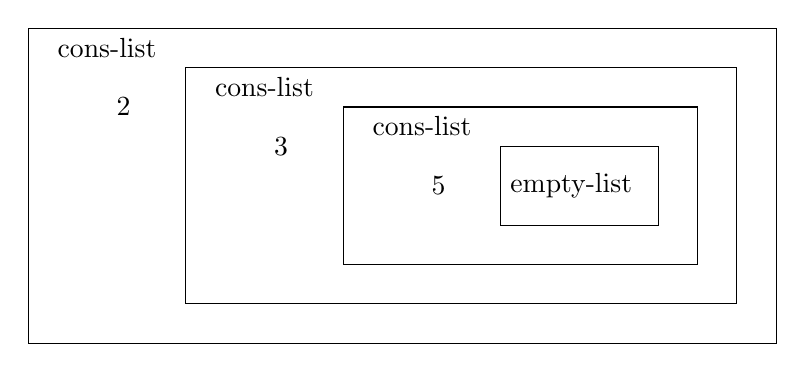
\begin{tikzpicture}
    \draw (0, 0) rectangle (9.5, 4); \node [below] at (1, 4)
    {\lstinline{cons-list}}; \node [right] at (1, 3) {\lstinline{2}};
    \draw (2, 0.5) rectangle (9, 3.5); \node [below] at (3, 3.5)
    {\lstinline{cons-list}}; \node [right] at (3, 2.5)
    {\lstinline{3}}; \draw (4, 1) rectangle (8.5, 3); \node [below] at
    (5, 3) {\lstinline{cons-list}}; \node [right] at (5, 2)
    {\lstinline{5}}; \draw (6, 1.5) rectangle (8, 2.5); \node [right]
    at (6, 2) {\lstinline{empty-list}};
  \end{tikzpicture}
  
  \caption{Struktur der Liste mit den Elementen 2 3 5}
  \label{fig:list-structure}
\end{figure}
%
\noindent An den Beispielen kann man sehen, dass es einen Unterschied
zwischen der intuitiven Struktur von Listen und ihrer Repräsentation
gibt. Intuitiv besteht eine Liste aus einer Aneinanderreihung ihrer
Elemente.  Die Repräsentation ist aber geschachtelt, wie
Abbildung~\ref{fig:list-structure} zeigt.  Sie erlaubt uns
insbesondere, aus kleineren Listen größere zu bauen und trotzdem die
kleineren Listen wiederzuverwenden:
%
\begin{lstlisting}
; Liste mit den Zahlen 1 2 3 5 7
(define list5 (cons 1 list4))
\end{lstlisting}
%
Dieses Beispiel zeigt außerdem, dass der Konstruktor \lstinline{cons} an eine
existierende Liste \emph{vorn} ein Element anhängt.

\label{sec:list-sum}
Nun sind wir bereit, eine Funktion über Listen zu schreiben, welche
die Zahlen einer Liste aufaddiert.  Kurzbeschreibung und Signatur
sehen so aus:
%
\begin{lstlisting}
; Summe der Elemente einer Liste von Zahlen berechnen
(: list-sum (list-of-numbers -> number))
\end{lstlisting}
%
Als Nächstes brauchen wir Testfälle, die wir mit Hilfe der
Beispiel-Listen von oben (und gegebenenfalls einem Taschenrechner)
konstruieren:
%
\begin{lstlisting}
(check-expect (list-sum list2) 5.85989)
(check-expect (list-sum list3) 6)
(check-expect (list-sum list4) 17)
\end{lstlisting}
%
\begin{aufgabeinline}
  Schreibe auch Testfälle für \lstinline{list-sum} auf Basis der
  Beispiel-Listen \lstinline{list0} und \lstinline{list1}!  Falls Du
  Dir nicht sicher bist, rate!
\end{aufgabeinline}
%
Als Nächstes kommt wie immer das Gerüst:
%
\begin{lstlisting}
(define list-sum
  (lambda (list)
    |\ldots|))
\end{lstlisting}
%
Die Signatur sagt, dass \lstinline{list-sum} eine Liste als Eingabe
akzeptiert~-- gemischte Daten.  Die Schablone dazu sieht so aus:
%
\begin{lstlisting}
(define list-sum
  (lambda (list)
    (cond
      ((empty? list) |\ldots|)
      ((cons? list) |\ldots|))))
\end{lstlisting}       
%
Beim \lstinline{cons-list}-Fall handelt es sich um zusammengesetzte
Daten, wir können also entsprechend der Schablone dafür
Selektor-Aufrufe hinschreiben.  Bei \lstinline{rest} sitzt außerdem
ein Selbstbezug, wir schreiben also auch einen rekursiven Aufruf in
die Schablone:
%
\begin{lstlisting}
(define list-sum
  (lambda (list)
    (cond
      ((empty? list) |\ldots|)
      ((cons? list)
       |\ldots|
       (first list)
       (list-sum (rest list))
       |\ldots|))))
\end{lstlisting}
%
Nun sind alle möglichen Konstruktionsanleitungen angewendet. Wir
vervollständigen die Schablone, zuerst den Fall für
Cons-Listen.  Dort steht in der Schablone \lstinline{(first list)} 
und \lstinline{(list-sum (rest list))}.  Zum Verständnis
hilft, die beiden Ausdrucke ins Deutsche zu übersetzen:
%
\begin{itemize}
\item \lstinline{(first list)} ist das \emph{erste Element der Liste} und
\item \lstinline{(list-sum (rest list))} ist die \emph{Summe der restlichen
    Elemente}.
\end{itemize}
%
Gefragt
ist aber die Summe \emph{aller Elemente}, dazu müssen wir die beiden
noch addieren:
%
\begin{lstlisting}
(+ (first list) (list-sum (rest list)))
\end{lstlisting}
%
Es bleibt der Fall der leeren Liste.  Intuitiv hat die gar keine
Summe, aber irgendetwas müssen wir da hinschreiben.  Wir schreiben 
vorläufig $0$ ins Programm, werden diese Wahl aber noch diskutieren:
%
\indexvariable{list-sum}
\begin{lstlisting}
(define list-sum
  (lambda (list)
    (cond
      ((empty? list) 0)
      ((cons? list)
       (+ (first list) (list-sum (rest list)))))))
\end{lstlisting}
%
Damit funktionieren die Testfälle und die Funktion ist fertig!

\begin{aufgabeinline}
  Verfolge die Auswertung der Testfälle im Stepper!
\end{aufgabeinline}

\begin{aufgabeinline}
  Ändere den Zweig für die leere Liste und schreibe etwas anderes als
  0 hin.  Funktionieren die Testfälle dann noch?
\end{aufgabeinline}
%
Tatsächlich ist $0$ die einzig richtige Zahl, die im
\lstinline{empty}-Fall stehen darf.  Das mag intuitiv einleuchten: die
leere Liste ist schließlich "<nichts"> und 0 ist auch irgendwie
"<nichts">.  Ein weiteres Beispiel wird aber gleich zeigen, dass diese
Argumentation zu einfach ist.

Wir schreiben als Nächstes eine Funktion, die alle Zahlen einer Liste
\emph{multipliziert}.   Hier sind Kurzbeschreibung, Signatur, Tests
und Gerüst:
%
\begin{lstlisting}
; Produkt der Elemente einer Liste von Zahlen berechnen
(: list-product (list-of-numbers -> number))

(check-expect (list-product list1) 42)
(check-expect (list-product list3) 6)
(check-expect (list-product list4) 210)

(define list-product
  (lambda (list)
    |\ldots|))
\end{lstlisting}
%
Die Schablone entsteht genau wie bei \lstinline{list-sum} aus den
Konstruktionsanleitungen für gemischte Daten, zusammengesetzte Daten
und Selbstbezüge:
%
\begin{lstlisting}
(define list-product
  (lambda (list)
    (cond
      ((empty? list) |\ldots|)
      ((cons? list)
       |\ldots|
       (first list) 
       |\ldots|
       (list-product (rest list))))))
\end{lstlisting}
%
Wir kümmern uns wieder zuerst um den
\lstinline{cons}-Fall. In der Schablone stehen \lstinline{(first list)}, das erste
Element und \lstinline{(list-product (rest list))}, das Produkt der
restlichen Elemente.  Wir müssen nur noch beide miteinander
multiplizieren, um das Produkt aller Elemente zu berechnen:
%
\begin{lstlisting}
(* (first list) (list-product (rest list)))
\end{lstlisting}
%
Bleibt wieder der \lstinline{empty}-Fall~-- wieder die leere Liste.
Die Versuchung ist groß, wieder "<nichts"> hinzuschreiben, also 0.
Dann allerdings schlagen \emph{alle} Testfälle fehl:
\begin{alltt}
Der tatsächliche Wert 0 ist nicht der erwartete Wert 42.
Der tatsächliche Wert 0 ist nicht der erwartete Wert 6.
Der tatsächliche Wert 0 ist nicht der erwartete Wert 210.
\end{alltt}
%
Warum kommt immer $0$ heraus?  Das können wir anhand der Auswertung
von
\lstinline{(list-product list3)}
sehen.  Die sieht so aus~-- wir haben
einige Zwischenschritte ausgelassen:
%
\begin{lstlisting}
(list-product list3)
|\evalsto| (list-product (cons 1 (cons 2 (cons 3 empty))))
|\evalsto| (cond ((empty? (cons 1 |\ldots|)) |\ldots|) ((cons? (cons 1 |\ldots|)) |\ldots|))
|\evalsto| (cond ((empty? (cons 1 |\ldots|)) |\ldots|) ((cons? (cons 1 |\ldots|)) |\ldots|))
|\evalsto| (* (first (cons 1 |\ldots|)) (list-product (rest (cons 1 |\ldots|))))
|\evalsto| (* 1 (list-product (rest (cons 1 |\ldots|))))
|\evalsto| (* 1 (list-product (cons 2 (cons 3 empty))))
|\evalsto| (* 1 (* 2 (list-product (cons 3 empty))))
|\evalsto| (* 1 (* 2 (* 3 (list-product empty))))
|\evalsto| (* 1 (* 2 (* 3 (cond ((empty? empty) 0) |\ldots|))))
|\evalsto| (* 1 (* 2 (* 3 (cond (#t 0) |\ldots|))))
|\evalsto| (* 1 (* 2 (* 3 0)))
\end{lstlisting}
%
Die Auswertung ist auf so einem guten Weg~-- aber um Schluss macht
\lstinline{list-product} alles kaputt und multipliziert mit $0$.  Und so
ist es mit \emph{jeder} Eingabe.  Wir müssten also
statt mit $0$ mit einer Zahl multiplizieren, die das Ergebnis nicht
kaputtmacht sondern genauso lässt, wie es ist.  Im Fall der
Multiplikation ist das die $1$, nicht die $0$.  Die richtige Funktion
sieht damit so aus:
%
\indexvariable{list-product}
\begin{lstlisting}
(define list-product
  (lambda (list)
    (cond
      ((empty? list) 1)
      ((cons? list)
       (* (first list) (list-product (rest list)))))))
\end{lstlisting}
%
Rückblickend können wir damit auch erklären, warum bei
\lstinline{list-sum} im \lstinline{empty}-Fall $0$ stehen muss: Die $0$
macht beim Addieren das Ergebnis nicht kaputt.  Darum spricht man auch
davon, dass $0$ das \textit{neutrale Element}\index{neutrales Element}
bezüglich der Addition ist, $1$ das neutrale Element bezüglich der
Multiplikation.\label{page:neutrales-element}

\section{Listen mit anderen Elementen}

\mentioncode{listen/list-of.rkt}
%
Das Prinzip "<Liste"> ist nicht auf Listen von Zahlen beschränkt:
Genauso gut kann man sich Listen aus Zeichenketten, den Tieren aus
Kapitel~\ref{sec:animal} oder Bildern vorstellen.  Um das zu
ermöglichen, können wir die Datendefinition
anpassen.  Wir entfernen alle Erwähnungen von
Zahlen und sprechen ausschließlich von "<Elementen">:
%
\begin{lstlisting}
; Eine Liste ist eins der folgenden:
; - eine leere Liste
; - eine Cons-Liste

; Eine Cons-Liste besteht aus:
; - dem ersten Element
; - einer Liste mit den restlichen Elementen
\end{lstlisting}
%
Tatsächlich können wir Listen bereits bauen, deren Elemente keine
Zahlen sind:
%
\indexvariable{string-list}
\begin{lstlisting}
(define string-list (cons "Mike" (cons "Sperber" empty)))
\end{lstlisting}
%
\begin{aufgabeinline}
  Probiere die Definition von \lstinline{string-list} aus!
\end{aufgabeinline}
%
Diese Definition kann DrRacket zwar ausführen, aber es gibt jede
Menge Signaturverletzungen.

Die verletzten Signaturen sind allesamt \lstinline{number}, am
prominentesten in der Record-Definition von \lstinline{cons-list}.
Wenn wir dort auch Zeichenketten verwenden wollen, ohne Listen aus
Zahlen zu verbieten, müssen wir über
\lstinline{number} und \lstinline{string} abstrahieren.  Bei der
Record-Definition geht das, indem wir aus \lstinline{cons-list} stattdessen
\lstinline{(cons-list-of element)} machen.
Das wirkt wie ein
\lstinline{lambda} mit \lstinline{element} als Parameter.  Wir können
dann \lstinline{element} innerhalb
der Record-Definition benutzen:\label{function:cons-list-of}
%
\indexvariable{cons-list-of}
\begin{lstlisting}
(define-record (cons-list-of element)
  cons
  cons?
  (first element)
  (rest  |\ldots|))
\end{lstlisting}
%
Diese Record-Definition definiert \lstinline{cons-list-of} als Funktion,
die eine Signatur akzeptiert (die Signatur der Elemente) und eine
Signatur zurückliefert, nämlich die der Cons-Listen mit der gegebenen
Signatur für die Elemente.  Die Signatur können wir auch hinschreiben:
%
\begin{lstlisting}
(: cons-list-of (signature -> signature))
\end{lstlisting}
%
Da \lstinline{cons-list-of} eine Signatur konstruiert, nennen wir diese
Funktion auch \textit{Signatur-Konstruktor}.\index{Signatur-Konstruktor}
Das \lstinline{element} ist ein \textit{Signatur-Parameter}\index{Signatur-Parameter}.
Wir müssen also immer da, wo wir vorher \lstinline{cons-list} stand,
\lstinline{(cons-list-of ...)} schreiben und eine Signatur für die
Elemente angeben, also zum Beispiel \lstinline{(cons-list-of number)}
oder \lstinline{(cons-list-of string)}.

Die Signatur von \lstinline{rest} war vorher
\lstinline{list-of-numbers}, die müssen wir also auch ändern.  Wie
genau, ergibt sich erst im Zusammenhang mit der abstrahierten
Definition von \lstinline{list-of-numbers}.  Da es sich hier um eine
ganz normale Definition mit \lstinline{define} handelt, können wir ein
\lstinline{lambda} benutzen, um über den Signatur der Elemente zu
abstrahieren:
%
\indexvariable{list-of}
\begin{lstlisting}
(define list-of
  (lambda (element)
    (signature
     (mixed empty-list
            (cons-list-of element)))))
\end{lstlisting}
%
Wir können mit dieser Definition nun statt \lstinline{list-of-numbers} also
\lstinline{(list-of number}) schreiben.  Damit können wir auch die
Record-Definition von \lstinline{cons-list-of} vervollständigen, indem
wir beim \lstinline{rest}-Feld als Signatur \lstinline{(list-of element)} schreiben, wo vorher
\lstinline{list-of-numbers} stand:
%
\begin{lstlisting}
(define-record (cons-list-of element)
  cons
  cons?
  (first element)
  (rest  (list-of element)))
\end{lstlisting}
%
Das erledigt die Signaturverletzungen.

\begin{feature}{\texttt{define-record} mit Signatur-Parametern}{scheme:define-record-parameters}
Eine \lstinline{define-record}"=Form\indexvariable{define-record}
mit Signatur-Parametern hat folgende allgemeine Gestalt:\label{def:define-record-parameters}
%
\begin{alltt}
(define-record (\(t\) \(\mathit{sp}\sb{1}\) \(\ldots\) \(\mathit{sp}\sb{k}\))
  \(c\)
  \(p\)
  (\(\mathit{sel}\sb{1}\) \(\mathit{sig}\sb{1}\))
  \(\ldots\)
  (\(\mathit{sel}\sb{n}\) \(\mathit{sig}\sb{n}\)))
\end{alltt}
%
%
\begin{itemize}
\item Die Signatur-Parameter $\mathit{sp}\sb{1} \ldots \mathit{sp}\sb{k}$
können in den Signaturen
\(\mathit{sig}\sb{1}\ldots\mathit{sig}\sb{n}\) verwendet werden.
\item $t$ ist der Name des Signatur-Konstruktors mit der Signatur:
  %
\begin{alltt}
(: \(t\) (signature \(\ldots\) \textrm{(\(k\)-mal)} -> signature))
\end{alltt}
  \item $c$, $p$ und $\mathit{sel}_1, \ldots, \mathit{sel}_n$ sind 
    die Namen von Konstruktor, Prädikat und Selektoren.
\end{itemize}
%
\end{feature}

Abbildung~\ref{scheme:define-record-parameters} fasst die
neue Form von \lstinline{define-record} mit
Signatur-Parametern zusammen.
Bei dieser neuen Form von \lstinline{define-record} ist
nicht mehr offensichtlich, wie die Signaturen des Konstruktors und der
beiden Selektoren aussehen sollen, wenn wir sie ausschreiben.  Wir
brauchen dafür ein neues Konstrukt, um auszudrücken, dass potenziell
bei jedem Aufruf von \lstinline{cons}, \lstinline{first} und
\lstinline{rest} eine andere Elementsignatur verwendet wird.  Das
sieht so aus:
%
\begin{lstlisting}
(: cons (%element (list-of %element) -> (cons-list-of %element)))
(: first ((cons-list-of %element) -> %element))
(: rest ((cons-list-of %element) -> (list-of %element)))
\end{lstlisting}
%
Das \verb|%| kennzeichnet
\textit{Signaturvariablen}\index{Signaturvariable}.  Die
Signaturvariable \lstinline{%element} steht für eine beliebige
Signatur.  Die Signatur-Deklaration von \lstinline{cons} bedeutet
außerdem, dass die Signatur von neuem Element (das erste \lstinline{%element})
und die Signatur der Listenelemente (das \lstinline{%element} in 
\lstinline{(list %element)} übereinstimmen sollten.  (DrRacket
  überprüft dies aber nicht.)

Vielleicht ist Dir der Gedanke gekommen, dass statt
\lstinline{%element} in den obigen Signaturen auch \lstinline{any}
stehen könnte.  Rein technisch gesehen ist das korrekt.  Allerdings
wären die resultierenden Signaturen weniger präzise.  Nimm einmal
an, dort stünde zum Beispiel das hier:
%
\begin{lstlisting}
(: cons (any (list-of any) -> (cons-list-of any)))
\end{lstlisting}
%
Diese Signatur sagt "<\lstinline{cons} akzeptiert irgendeinen Wert und
irgendeine Liste und produziert wieder irgendeine Liste">.  Zum
Vergleich sagt die Signatur
%
\begin{lstlisting}
(: cons (%element (list-of %element) -> (cons-list-of %element)))
\end{lstlisting}
%
aus, dass das neue Element, das \lstinline{cons} akzeptiert, die
gleiche Signatur erfüllen muss wie die schon vorhandenen Elemente der
Liste und die Elemente der Resultatliste: Alle drei Vorkommen von \lstinline{%element} müssen in einer
konkreten Anwendung von \lstinline{cons} die gleiche Signatur sein.

Bevor das Programm wieder
funktioniert, müssen wir noch ein kleines Problem
beheben:

\lstinline{List-of-numbers} ist nicht mehr
definiert, steht aber noch in den Signatur"=Deklarationen von
\lstinline{list-sum} und \lstinline{list-product}.  Wir können
entweder \lstinline{list-of-numbers} durch \lstinline{(list-of number)}
ersetzen oder eine Signatur-Definition
dazuschreiben:
%
\indexvariable{list-of-numbers}
\begin{lstlisting}
(define list-of-numbers (signature (list-of number)))
\end{lstlisting}
%
Diese Definition muss vor \lstinline{list-sum}
und \lstinline{list-product} stehen, damit sie dort bekannt ist.

\section{Konstruktionsanleitung}

Bei der Konstruktion von Funktionen, die Listen akzeptieren, haben wir
drei Schablonen kombiniert: gemischte und
zusammengesetzte Daten sowie Selbstbezüge.  Wir
werden noch viele Funktionen mit Listen als Eingabe schreiben.
Deshalb lohnt es sich, solchen Funktionen eine eigene
Konstruktionsanleitung zu widmen:

\begin{konstruktionsanleitung}{Listen als Eingabe: Schablone}
  \label{ka:listen-eingabe-schablone}
Die Schablone für eine Funktion, die eine Liste akzeptiert, sieht
folgendermaßen aus:
%
\begin{lstlisting}
(: |\(f\)| (... (list-of |\(\mathit{elem}\)|) ... -> ...))

(define |\(f\)|
  (lambda (|\ldots| |\(\mathit{list}\)| |\ldots|)
    (cond
      ((empty? |\(\mathit{list}\)|) |\ldots|)
      ((cons? |\(\mathit{list}\)|)
       |\ldots|
       (first |\(\mathit{list}\)|)
       |\ldots|
       (|\(f\)| |\ldots| (rest |\(\mathit{list}\)|) |\ldots|)
       |\ldots|
       ))))
\end{lstlisting}
  
  
\end{konstruktionsanleitung}

\section{Eingebaute Listen}

Da Listen in diesem Buch noch oft vorkommen und es umständlich ist,
jedesmal die Definitionen für \lstinline{cons} und \lstinline{list-of} an
den Anfang von Programmen zu setzen, macht die nächste Sprachebene das
Programmieren mit Listen einfacher.\index{Sprachebene}

\smallskip

\noindent\textbf{Schalte deshalb in die nächste Sprachebene hoch:}

\smallskip

\noindent Fange eine neue Datei an.  Wähle danach wieder das Menü
\texttt{Sprache} aus, darunter den Menüpunkt \texttt{Sprache auswählen} und dann
\texttt{Schreibe Dein Programm!} (\emph{ohne} \texttt{Anfänger}).
Dann drücke noch einmal \texttt{Start}.

\begin{feature}{\texttt{list}}{scheme:list}
  Die eingebaute Funktion \lstinline{list}\indexvariable{list} erlaubt es, Listen aus ihren Elementen
  ohne Verwendung von \lstinline{cons} zu erzeugen.  Sie
  akzeptiert eine beliebige Anzahl von Argumenten, macht daraus eine
  Liste und gibt diese zurück:
%
\begin{lstlisting}
(list 1 2 3)
|\evalsto| #<list 1 2 3>
(list "Axl" "Slash" "Izzy")
|\evalsto| #<list "Axl" "Slash" "Izzy">
\end{lstlisting}
\end{feature}

Ab sofort sind \lstinline{cons}, \lstinline{cons?}, \lstinline{first} und
\lstinline{rest} vordefiniert genau wie der Signaturkonstruktor
\lstinline{list-of}.  Es gibt außerdem eine praktische neue Funktion
\lstinline{list}, die in Abbildung~\ref{scheme:list} beschrieben ist.

In der neuen Sprachebene werden nichtleere Listen übersichtlicher ausgedruckt
als bisher, nämlich als
\lstinline{#<list ...>}, wobei die Listenelemente zwischen den spitzen
Klammern aufgereiht sind:
%
\begin{lstlisting}
(list "Axl" "Slash" "Izzy")
|\evalsto| #<list "Axl" "Slash" "Izzy">
\end{lstlisting}
%

\section{Parametrische Polymorphie}
\label{sec:parametric-polymorphism}
\label{sec:more-lists}

\mentioncode{listen/polymorphism.rkt}
%
Keine Angst vor der hochtrabenden Überschrift: Wir schreiben in diesem
Abschnitt eine recht einfache Funktion, welche die Länge einer Liste
ermittelt.\indexvariable{list-length} Hier ist die
Kurzbeschreibung:
%
\begin{lstlisting}
; Länge einer Liste berechnen
\end{lstlisting}
%
Der Anfang einer Signatur-Deklaration sieht so aus:
%
\begin{lstlisting}
(: list-length ((list-of |\ldots|) -> natural))
\end{lstlisting}
%
Was können wir anstelle der Ellipse hinschreiben?  Der Funktion sollte
egal sein, auf welche Signatur die Elemente der Liste passen. Wir
können dies zum Ausdruck bringen, indem wir eine Signaturvariable
verwenden, genau wie bei den Signaturen von \lstinline{cons},
\lstinline{first} und \lstinline{rest}.  Das sieht so aus:\label{page:list-length}
%
\begin{lstlisting}
(: list-length ((list-of %element) -> natural))
\end{lstlisting}
%
Die Verwendung der Signaturvariable \lstinline{%element} bedeutet,
genau wie oben, dass die Signatur der Elemente der Liste bei jedem
Aufruf von \lstinline{list-length} anders sein kann.

Solche Funktionen, die Argumente akzeptieren, deren Signaturen
Signaturvariablen enthalten, heißen \textit{polymorph} oder auch
\textit{parametrisch polymorph} (weil die Signaturvariable eine Art
Parameter abgibt), und das dazugehörige Konzept heißt
\textit{parametrische
  Polymorphie}\index{Polymorphie}\index{parametrische Polymorphie}:
ein großes Wort, das hier für eine kleine Sache steht.  Mehr und interessantere
Beispiele für parametrische Polymorphie wird es in
Kapitel~\ref{cha:higher-order} geben.

Weiter mit \texttt{list-length}~-- hier ist das Gerüst:
%
\begin{lstlisting}
(define list-length
  (lambda (lis)
    |\ldots|))
\end{lstlisting}
%
Die Schablone ist wie gehabt:
%
\begin{lstlisting}
(define list-length
  (lambda (lis)
    (cond
      ((empty? lis) |\ldots|)
      ((cons? lis) 
       |\ldots| (first lis) |\ldots|
       |\ldots| (list-length (rest lis)) |\ldots|))))
\end{lstlisting}
%
Es ist \texttt{list-length} egal, was der Wert von \texttt{(first
  lis)} ist.  Die Länge der Liste ist unabhängig davon, was für Werte
sich darin befinden~-- entscheidend ist nur, wieviele es sind.  (Dieser
Umstand ist gerade verantwortlich für die parametrische Polymorphie.)
Deshalb können wir den Selektoraufruf \texttt{(first lis)} aus der Schablone streichen und
diese dann zum vollständigen Rumpf ergänzen:
%
\indexvariable{list-length}
\begin{lstlisting}
(define list-length
  (lambda (lis)
    (cond
      ((empty? lis) 0)
      ((cons? lis) 
       (+ 1 
          (list-length (rest lis)))))))
\end{lstlisting}
%
Die Funktion~\lstinline{list-length} ist unter dem
Namen~\lstinline{length}\indexvariable{length} fest
eingebaut.\label{func:length}

\section{Funktionen, die Listen produzieren}

\mentioncode{listen/dillo-list.rkt}
%
In den vorherigen Abschnitten haben wir ausschließlich Funktionen
programmiert, die Listen \emph{akzeptieren}.  In diesem Abschnitt
schreiben wir Funktionen, die Listen \emph{produzieren}.  Das geht mit
Techniken, die wir bereits vorgestellt haben.  Wir machen die Sache
interessanter, indem wir in einem ersten Beispiel Listen von
zusammengesetzten Daten betrachten und in einem zweiten Beispiel zwei
Listen verarbeiten.

\subsection{Gürteltiere überfahren}

Auf Seite~\pageref{page:run-over-dillo} haben wir die Funktion
\texttt{run-over-dillo} geschrieben, die für das Überfahren von
Gürteltieren zuständig ist.  In diesem Abschnitt schreiben wir die
Funktion, die das gleich massenweise erledigt, beispielsweise für alle
Gürteltiere auf einem Highway.

Dazu übernehmen wir Daten- und Record-Definition von Gürteltieren aus
Abschnitt~\ref{page:run-over-dillo} sowie die Funktiondefinition von
\lstinline{run-over-dillo}.  Du kannst auch einfach den Gürteltier-Code
erweitern~-- dann musst Du allerdings die Sprachebene auf
\texttt{Schreibe Dein Programm!} hochschalten, damit die Listen zur
Verfügung stehen.

Gürteltiere können wir in Listen stecken, ebenso wie Zahlen,
Zeichenketten oder boolesche Werte.  Hier ist ein Beispiel:
%
\indexvariable{highway75}
\begin{lstlisting}
; Gürteltiere auf Highway 75
(define highway75 (list dillo1 dillo2 dillo3 dillo4))
\end{lstlisting}
(\lstinline{Dillo1}, \lstinline{dillo2}, \lstinline{dillo3} und \lstinline{dillo4} sind die
Beispielgürteltiere aus Abschnitt~\ref{page:run-over-dillo}.)

Diese Liste hat die Signatur \lstinline{(list-of dillo)}.  Wenn wir eine
Funktion schreiben wollen, die alle Gürteltiere aus einer Liste
überfährt, müsste diese also folgende Kurzbeschreibung und Signatur
haben:
%
\begin{lstlisting}
; Gürteltiere überfahren
(: run-over-dillos ((list-of dillo) -> (list-of dillo)))
\end{lstlisting}
%
Als Testfall kann obige Beispielliste herhalten:
%
\begin{lstlisting}
(check-expect (run-over-dillos highway75)
              (list (make-dillo 55000 #f)
                    dillo2
                    (make-dillo 60000 #f)
                    dillo4))
\end{lstlisting}
%
Zur Erinnerung: \lstinline{dillo2} und \lstinline{dillo4} sind bereits tot,
dementsprechend sind sie überfahren wie zuvor.
Hier ist das Gerüst:
%
\begin{lstlisting}
(define run-over-dillos
  (lambda (dillos)
    |\ldots|))
\end{lstlisting}
%
Die Funktion akzeptiert eine Liste als Eingabe, wir können also, wie
schon so oft, die entsprechende Schablone zum Einsatz bringen:
%
\begin{lstlisting}
(define run-over-dillos
  (lambda (dillos)
    (cond
     ((empty? dillos) |\ldots|)
     ((cons? dillos)
      |\ldots| (first dillos) |\ldots|
      |\ldots| (run-over-dillos (rest dillos)) |\ldots|))))
\end{lstlisting}
%
Im ersten Zweig ist die Sache klar: Geht eine leere Liste rein, kommt
auch eine leere Liste raus.  Im zweiten Zweig können wir uns erst
einmal um das erste Gürteltier kümmern.  Wir haben ja bereits eine
Funktion, die ein einzelnes Gürteltier überfährt; diese können wir auf
das erste Element der Liste anwenden:
%
\begin{lstlisting}
(define run-over-dillos
  (lambda (dillos)
    (cond
     ((empty? dillos) empty)
     ((cons? dillos)
      |\ldots| (run-over-dillo (first dillos)) |\ldots|
      |\ldots| (run-over-dillos (rest dillos)) |\ldots|))))
\end{lstlisting}
%
Lesen wir noch einmal die beiden Ausdrücke, die im zweiten Zweig
stehen:
%
\begin{itemize}
\item \lstinline{(run-over-dillo (first dillos))} ist das erste Gürteltier
  der Liste, überfahren.
\item \lstinline{(run-over-dillos (rest dillos))} ist eine Liste der
  restlichen Gürteltiere, auch überfahren.
\end{itemize}
%
Gefragt ist eine Liste \emph{aller} Gürteltiere, überfahren:
Wir müssen also nur die Resultate der beiden Ausdrucke mit
\lstinline{cons} kombinieren:
%
\indexvariable{run-over-dillos}
\begin{lstlisting}
(define run-over-dillos
  (lambda (dillos)
    (cond
     ((empty? dillos) empty)
     ((cons? dillos)
      (cons (run-over-dillo (first dillos))
            (run-over-dillos (rest dillos)))))))
\end{lstlisting}
%
Fertig!

Dieses Beispiel zeigt, dass wir für Funktionen, die Listen produzieren,
keine neue Technik brauchen: Wenn eine Funktion eine leere Liste
produzieren soll, benutzen wir an der entsprechenden Stelle
\lstinline{empty}, und bei nichtleeren Listen benutzen wir
\lstinline{cons}, bringen also die Schablone für Funktionen zum
Einsatz, die zusammengesetzte Daten produzieren.

\subsection{Gürteltiere extrahieren}

Wir nehmen uns noch eine weitere Übung vor, bei der Listen produziert
werden: Aus einer Liste von Gürteltieren wollen wir alle (noch)
lebenden herausholen, vielleicht, um sie in Sicherheit zu bringen.

So sehen Kurzbeschreibung, Signatur, ein Testfall und Gerüst aus:
%
\begin{lstlisting}
; Lebendige Gürteltiere aufsammeln
(: live-dillos ((list-of dillo) -> (list-of dillo)))

(check-expect (live-dillos highway75)
              (list dillo1 dillo3))

(define live-dillos
  (lambda (dillos)
    |\ldots|))
\end{lstlisting}
%
Wir fügen als Nächstes die Standard-Schablone für Funktionen ein, die
Listen akzeptieren:
%
\begin{lstlisting}
(define live-dillos
  (lambda (dillos)
    (cond
      ((empty? dillos) |\ldots|)
      ((cons? dillos)
       |\ldots| (first dillos) |\ldots|
       |\ldots| (live-dillos (rest dillos)) |\ldots|))))
\end{lstlisting}
%
Der erste
Fall betrifft die leere Liste~-- aus einer leeren Liste von
Gürteltiere können wir keine lebendigen Gürteltiere herausholen,
da kommt also \lstinline{empty} hin.
Im zweiten Fall ist es etwas aufwendiger.  Wir machen uns wieder klar,
was die beiden Bestandteile bedeuten, die in der Schablone stehen:
%
\begin{itemize}
\item \lstinline{(first dillo)} ist das erste Gürteltier in der Liste.
\item \lstinline{(live-dillos (rest dillos))} sind die lebendigen
  unter den restlichen Gürteltieren.
\end{itemize}
%
Da die Gesamtaufgabe ist, die lebendigen Gürteltiere
zu extrahieren, sollten wir beim ersten Gürteltier feststellen, ob
es (noch) lebt.  Da steht dann folgender Zwischenstand:
%
\begin{lstlisting}
(define live-dillos
  (lambda (dillos)
    (cond
      ((empty? dillos) empty)
      ((cons? dillos)
       |\ldots| (dillo-alive? (first dillos)) |\ldots|
       |\ldots| (first dillos) |\ldots|
       |\ldots| (live-dillos (rest dillos)) |\ldots|))))
\end{lstlisting}
%
Der Aufruf \lstinline{(dillo-alive? (first dillos))} bietet sich 
für eine binäre Verzweigung an:
%
\begin{lstlisting}
(define live-dillos
  (lambda (dillos)
    (cond
      ((empty? dillos) empty)
      ((cons? dillos)
       (if (dillo-alive? (first dillos))
           |\ldots|
           |\ldots|)
       |\ldots| (first dillos) |\ldots|
       |\ldots| (live-dillos (rest dillos)) |\ldots|))))
\end{lstlisting}
%
Wir müssen uns jetzt überlegen, was wir in die beiden Zweige des
\lstinline{if} schreiben.  Im ersten Zweig~-- der Konsequente~--  ist
das Gürteltier \lstinline{(first dillos)} (noch) am Leben, im
zweiten~-- der Alternative~-- ist es tot.

In der Alternative (Gürteltier tot) ist \lstinline{(live-dillos (rest dillos))} schon
die richtige Antwort.  \lstinline{(first dillos)} fällt unter den Tisch:
%
\begin{lstlisting}
(define live-dillos
  (lambda (dillos)
    (cond
      ((empty? dillos) empty)
      ((cons? dillos)
       (if (dillo-alive? (first dillos))
           |\ldots|
           (live-dillos (rest dillos)))
       |\ldots| (first dillos) |\ldots|))))
\end{lstlisting}
%
Auch, wenn wir den rekursiven Aufruf \lstinline{(live-dillos (rest dillos))}
scheinbar schon "<verbraucht"> haben~-- im  anderen Zweig (Gürteltier lebt
(noch)) brauchen wir die restlichen lebendigen Gürteltiere noch
einmal.  Wir müssen diesmal aber darauf achten, dass wir das erste
Gürteltier in der Ausgabe wieder unterbringen und vorn an die
restlichen Gürteltiere dran-\lstinline{cons}-en:\label{page:live-dillos}
%
\indexvariable{live-dillos}
\begin{lstlisting}
(define live-dillos
  (lambda (dillos)
    (cond
      ((empty? dillos) empty)
      ((cons? dillos)
       (if (dillo-alive? (first dillos))
           (cons (first dillos)
                 (live-dillos (rest dillos)))
           (live-dillos (rest dillos)))))))
\end{lstlisting}
%
Fertig!

\subsection{Zwei Listen aneinanderhängen}
\label{sec:concatenate}
In unserem nächsten Beispiel ist eine Funktion
\lstinline{concatenate}\indexvariable{concatenate} gefragt, die zwei
Listen aneinanderhängt.
% 
%
Kurzbeschreibung, Signatur und Gerüst sehen folgendermaßen aus:\indexvariable{concatenate}
%
\begin{lstlisting}
; zwei Listen aneinanderhängen
(: concatenate ((list-of %element) (list-of %element) 
               -> (list-of %element)))
\end{lstlisting}
%
Diese Funktion ist wie \lstinline{list-length} polymorph~-- in der
Signatur kommt die Signaturvariable \lstinline{%element} vor.
Beachte, dass \lstinline{%element} \emph{dreimal} vorkommt: Die
Signatur besagt, dass die Signaturen der Elemente der beiden
Eingabelisten und die Signatur der Ausgabeliste sich einander entsprechen.
Hier sind Testfall und Gerüst für \lstinline{concatenate}:
% 
\begin{lstlisting}
(check-expect (concatenate (list 1 2 3) (list 4 5 6))
              (list 1 2 3 4 5 6))

(define concatenate
  (lambda (list1 list2)
    |\ldots|))
\end{lstlisting}
%
Konstruktionsanleitung~\ref{ka:listen-eingabe-schablone} auf Seite~\pageref{ka:listen-eingabe-schablone} ist
eigentlich nur für Funktionen gedacht, die eine einzelne Liste
akzeptieren.  Welche von beiden ist das $\mathit{list}$ aus der Anleitung?  Im
Zweifelsfall können wir beide Alternativen ausprobieren.  Wir
versuchen es zunächst mit \lstinline{list2}:
%
\begin{lstlisting}
(define concatenate
  (lambda (list1 list2)
    (cond
      ((empty? list2) |\ldots|)
      ((cons? list2) 
       |\ldots| (first list2) |\ldots|
       |\ldots| (concatenate list1 (rest list2)) |\ldots|))))
\end{lstlisting}
%
Der erste Zweig des \lstinline{cond} ist noch einfach: Wenn
\lstinline{list2} leer ist, muss \lstinline{list1} herauskommen.  Jedoch wäre für
das obige Beispiel der Wert von \lstinline{(concatenate list1 (rest list2))}
die Liste \lstinline{#<list 1 2 3 5 6>}.
Bei dieser Liste fehlt das
Element 4 in der Mitte, und es ist nicht ersichtlich, wie unsere Funktion
sie passend ergänzen könnte.  Diese
Möglichkeit führt also in eine Sackgasse. Wir versuchen deshalb, die Schablone  auf
\lstinline{list1} 
 statt auf \lstinline{list2} anzuwenden:
%
\begin{lstlisting}
(define concatenate
  (lambda (list1 list2)
    (cond
      ((empty? list1) |\ldots|)
      ((cons? list1) 
       |\ldots| (first list1) |\ldots|
       |\ldots| (concatenate (rest list1) list2) |\ldots|))))
\end{lstlisting}
%
Die erste Ellipse ist einfach zu ersetzen:  Ist die erste Liste
leer, ist das Ergebnis die zweite Liste \lstinline{list2}.  Für den
zweiten Fall sollten wir uns noch einmal ins Gedächtnis rufen,
was für einen Wert \lstinline{(concatenate (rest list1) list2)} liefert: das Ergebnis
dieses Aufrufs ist eine
Liste, die aus \lstinline{(rest list1)} und \lstinline{list2} zusammengesetzt
wurde.  Auf das obige Beispiel übertragen, falls \lstinline{list1} die Liste
\lstinline{#<list 1 2 3>} ist und \lstinline{list2} die Liste
\lstinline{#<list 4 5 6>}, hat \lstinline{(rest list1)} den Wert \lstinline{#<list 2 3>}.
Der Wert von \lstinline{(concatenate (rest list1) list2)} wäre
also:
%
\begin{lstlisting}
#<list 2 3 4 5 6>
\end{lstlisting}
%
Es fehlt das erste Element von \lstinline{list1}, \lstinline{(first list1)}, 
das vorn an das Ergebnis angehängt werden muss.  Das geht
mit \lstinline{cons}:
%
\indexvariable{concatenate}
\begin{lstlisting}
(define concatenate
  (lambda (list1 list2)
    (cond
      ((empty? list1) list2)
      ((cons? list1) 
       (cons (first list1)
             (concatenate (rest list1) list2))))))
\end{lstlisting}
%
Dieses Beispiel zeigt ein weiteres Schablonenelement, das noch öfter
vorkommen wird:  Wie bei anderen zusammengesetzten Daten müssen Funktionen, die
Listen konstruieren sollen, irgendwo ein \lstinline{cons} enthalten.

Da viele Programme die Funktionen \lstinline{list-length} und
\lstinline{concatenate} benötigen,
sind sie in den Lehrsprachen  übrigens bereits unter den Namen
\lstinline{length}\indexvariable{length} und
\lstinline{append}\indexvariable{append} eingebaut.


\section{Minimum einer Liste und lokale Variablen}
\label{sec:list-min}

\mentioncode{listen/list-min.rkt}
%
Wir nehmen uns noch eine weitere Übung vor, nämlich das Minimum einer
Liste von Zahlen zu berechnen.  Das ist scheinbar einfach, birgt aber
einige Untiefen.  Hier sind der erste Anlauf für Kurzbeschreibung,
Tests und Gerüst:
%
\begin{lstlisting}
; Minimum einer Liste von Zahlen berechnen
(: list-min ((list-of real) -> real))

(check-expect (list-min (list 5 3 1 4)) 1)
(check-expect (list-min (list 5 3 1 4 -4 3)) -4)
\end{lstlisting}
%
Vielleicht siehst Du schon das erste Problem.  Die Tests sparen einen
einfachen aber wichtigen Fall aus, nämlich die leere Liste~-- und die
hat kein Minimum.

Eine Möglichkeit wäre, in dem Fall \lstinline{violation} aufzurufen
wie in Abschnitt~\ref{sec:violation} auf
Seite~\pageref{sec:violation}.  (Siehe dazu
Aufgabe~\ref{aufgabe:list-min-violation} auf
Seite~\pageref{aufgabe:list-min-violation}.)  Eine andere ist, wie in
Abschnitt~\ref{sec:maybe} auf Seite~\pageref{sec:maybe} einen
Extra-Wert für diesen Fall zu benutzen.  Das hat wie dort den Vorteil,
dass wir in der Signatur ablesen können, dass die Funktion auch
fehlschlagen kann.  Wir führen also folgenden leeren Record-Typ dafür
ein:
%
\begin{lstlisting}
; Kein Resultat
(define-record no-result
  make-no-result
  no-result?)
\end{lstlisting}
%
Die Signatur erweitern wir entsprechend:
%
\begin{lstlisting}
(: list-min ((list-of real) -> (mixed real no-result)))
\end{lstlisting}
%
Außerdem schreiben wir noch einen Testfall dafür:
%
\begin{lstlisting}
(check-expect (no-result? (list-min empty)) #t)
\end{lstlisting}
%
Nun können wir wie gewohnt die Schablone für Listen anwenden:
%
\begin{lstlisting}
(define list-min
  (lambda (list)
    (cond
      ((empty? list) ...)
      ((cons? list)
       ... (first list) ...
       ... (list-min (rest list)) ...))))
\end{lstlisting}
%
Der \lstinline{empty}-Fall ist gerade der, in dem es kein Resultat
gibt:
%
\begin{lstlisting}
(define list-min
  (lambda (list)
    (cond
      ((empty? list) (make-no-result))
      ((cons? list)
       ... (first list) ...
       ... (list-min (rest list)) ...))))
\end{lstlisting}
%
Im \lstinline{cons}-Fall müssen wir darauf achten, dass der rekursive
Aufruf von \lstinline{list-min} gemischte Daten liefert.  Wir müssen
also eine Verzweigung einbauen, die zwischen \lstinline{no-result} und
einer Zahl unterscheidet.  Wir machen das mit einer binären Verzweigung:
%
\begin{lstlisting}
(define list-min
  (lambda (list)
    (cond
      ((empty? list) (make-no-result))
      ((cons? list)
       (if (no-result? (list-min (rest list)))
           ...
           ...)
       ... (first list) ...
       ... (list-min (rest list)) ...))))
\end{lstlisting}
%
Falls der rekursive Aufruf ein \lstinline{no-result} liefert, haben
wir nur das erste Element der Liste \lstinline{(first list)} in der
Hand~-- der Rest der Liste muss dann ja leer sein.  In dem Fall muss
\lstinline{(first list)} auch das Minimum sein:
%
\begin{lstlisting}
(define list-min
  (lambda (list)
    (cond
      ((empty? list) (make-no-result))
      ((cons? list)
       (if (no-result? (list-min (rest list)))
           (first list)
           ...)
       ... (first list) ...
       ... (list-min (rest list)) ...))))
\end{lstlisting}
%
Falls der rekursive Aufruf von \lstinline{list-min} ein Resultat
liefert, ist dieses Resultat das Minimum der restlichen Liste.
Um das Minimum der Gesamtliste zu berechnen, müssen wir es allerdings
noch mit \lstinline{(first list)} vergleichen, das ebenfalls das
Minimum sein könnte.  Abhängig vom Ergebnis des Vergleichs ist das
eine oder das andere das Minimum:
%
\begin{lstlisting}
(define list-min
  (lambda (list)
    (cond
      ((empty? list) (make-no-result))
      ((cons? list)
       (if (no-result? (list-min (rest list)))
           (first list)
           (if (< (first list)
                  (list-min (rest list)))
               (first list)
               (list-min (rest list))))))))
\end{lstlisting}
%
Diese Funktion ist korrekt.

Allerdings hat sie noch einen Makel: \lstinline{(list-min (rest list))}
taucht insgesamt dreimal auf, und es ist tatsächlich
möglich, dass alle drei tatsächlich ausgewertet werden: Dreimal die
gleiche Arbeit.  (Du kannst Dich mit dem Stepper davon überzeugen.)
Wir sollten dafür sorgen, dass der rekursive Aufruf nur einmal
ausgewertet wird.  Dazu führen wir ein neues Programmierkonstrukt ein,
die \textit{lokale Variable}\index{lokale
  Variable}\index{Definition!lokal} (siehe Abbildung~\ref{scheme:local-definition}), für die zunächst
eine Definition innerhalb des Rumpfes von \lstinline{list-min} anlegen:
%
\begin{lstlisting}
(define list-min
  (lambda (list)
    (cond
      ((empty? list) (make-no-result))
      ((cons? list)
       (define rest-min (list-min (rest list)))
       ...))))
\end{lstlisting}
%
\begin{feature}{lokale Definition, lokale Variable}{scheme:local-definition}
  Im Rumpf eines \lstinline{lambda} und im Zweig eines
  \lstinline{cond} kann jeweils am Anfang eine Definition stehen.
  Eine solche \textit{lokale Definition}\index{Definition!lokal}
  bindet eine \textit{lokale Variable}\index{lokale Variable}.

  Diese Definition wir jedesmal ausgewertet, wenn die Auswertung beim
  Rumpf des \lstinline{lambda} beziehungsweise beim Zweig des
  \lstinline{cond} ankommt und ist auch nur innerhalb davon
  ("<lokal">) sichtbar.
\end{feature}
%
Diese Definition wird jedesmal ausgewertet, wenn die Auswertung den
\lstinline{cond}-Zweig für \lstinline{cons} erreicht und ist auch nur
innerhalb dieses Zweiges aktiv.  Wir ersetzen nun 
\lstinline{(list-min (rest list))}
durch die neue Variable
\lstinline{rest-min}:
%
\begin{lstlisting}
(define list-min
  (lambda (list)
    (cond
      ((empty? list) (make-no-result))
      ((cons? list)
       (define rest-min (list-min (rest list)))
       (if (no-result? rest-min)
           (first list)
           (if (< (first list)
                  rest-min)
               (first list)
               rest-min))))))
\end{lstlisting}
%
Fertig!

Das heißt~\ldots ein kleines bißchen verbessern können wir sie noch:
Der \lstinline{if}-Ausdruck am Ende berechnet das Minimum von
\lstinline{(first list)} und \lstinline{rest-min}.  Für die Berechnung
des Minimums zweier Zahlen gibt es schon eine eingebaute Funktion
namens \lstinline{min}, die wir verwenden können:
%
\indexvariable{list-min}
\begin{lstlisting}
(define list-min
  (lambda (list)
    (cond
      ((empty? list) (make-no-result))
      ((cons? list)
       (define rest-min (list-min (rest list)))
       (if (no-result? rest-min)
           (first list)
           (min (first list) rest-min))))))
\end{lstlisting}
%
Jetzt aber fertig!

\section{Funktionen auf nichtleeren Listen}
\label{sec:list-min-nonempty}

Das \lstinline{list-min}-Beispiel war nützlich, um zu demonstrieren,
wie wir "<es gibt kein Ergebnis"> repräsentieren können.  Es gibt aber
noch eine andere Möglichkeit, mit dem Problem der leeren Liste bei
\lstinline{list-min} fertigzuwerden: Wir verbieten sie einfach!  Dann
brauchen wir \lstinline{no-result} gar nicht mehr.

Wir definieren also eine alternative Version von \lstinline{list-min}
mit Kurzbeschreibung und Signatur wie folgt:
%
\begin{lstlisting}
; Minimum einer nichtleeren Liste von Zahlen berechnen
(: list-min-nonempty ((cons-list-of real) -> real))
\end{lstlisting}
%
Der Signaturkonstruktor \lstinline{cons-list-of} entspricht dem
gleichnamigen Signatur-Konstruktor aus
Abschnitt~\ref{function:cons-list-of} und beschreibt Cons-Listen~--
das sind ja genau die nichtleeren.

Wir benutzen die gleichen Testfälle wie vorhin:
%
\begin{lstlisting}
(check-expect (list-min-nonempty (list 5 3 1 4)) 1)
(check-expect (list-min-nonempty (list 5 3 1 4 -4 3)) -4)
\end{lstlisting}
%
Die Schablone müssen wir gegenüber der für \lstinline{list-of}
allerdings etwas anpassen.  Schließlich liefert für eine nichtleere
Liste die Bedingung \lstinline{(empty? list)} \emph{immer}
\lstinline{#f} und \lstinline{(empty? list)} \emph{immer}
\lstinline{#t}, die Verzweigung damit wäre also sinnlos.  Es ist
stattdessen \lstinline{(rest list)}, das entweder leer oder nichtleer
sein kann.  Das sieht dann so aus:\label{func:list-min-nonempty}
%
\begin{lstlisting}
(define list-min-nonempty
  (lambda (list)
    (cond
      ((empty? (rest list)) ...)
      ((cons? (rest list))
       ... (first list) ...
       ... (list-min-nonempty (rest list)) ...))))
\end{lstlisting}
%
Im ersten Zweig hat die Liste also genau ein Element, im zweiten Zweig
hat sie mindestens zwei Elemente.  Das Minimum einer Liste mit einem
Element ist einfach dieses eine Element.  Im zweiten Fall können wir,
genau wie bei \lstinline{list-min}, das Minimum von
\lstinline{(first list)} und dem Minimum des Rests der Liste
berechnen:
%
\indexvariable{list-min-nonempty}
\begin{lstlisting}
(define list-min-nonempty
  (lambda (list)
    (cond
      ((empty? (rest list))
       (first list))
      ((cons? (rest list))
       (min (first list)
            (list-min-nonempty (rest list)))))))
\end{lstlisting}
%
Fertig!

\begin{aufgabeinline}
  Kannst Du vorhersagen, was genau passiert, wenn Du
  \lstinline{list-min-nonempty} trotzdem auf eine leere Liste
  anwendest?  Probiere es aus!
\end{aufgabeinline}

\begin{aufgabeinline}
  Schreibe eine spezielle Konstruktionsanleitung für Funktionen, die
  nichtleere Listen akzeptieren!
\end{aufgabeinline}

\section*{Anmerkungen}

Listen sind eine Art Alleskleber:
Sie taugen auch für die Repräsentation von Tabellen,
Mengen und vielen anderen zusammengesetzten Daten.  Für Listen gibt es
eine riesige Anzahl praktischer Funktionen, von denen die Funktionen in
diesem Kapitel nur die Spitze des Eisberges sind.  Da 
ab hier Listen in den Lehrsprachen fest eingebaut sind, können sie als universelles
Kommunikationsmittel zwischen Programmen dienen, weil sich Funktionen
auf Listen aus einem Programm auch in einem anderen verwenden lassen.
Dies unterscheidet funktionale Sprachen von vielen anderen Programmiersprachen, in
denen Listen vom Programmierer selbst definiert werden müssen oder nur
eine untergeordnete Rolle spielen.

\section*{Aufgaben}

\begin{aufgabe}
  Schreibe Ausdrücke für Listen, welche die Beispiellisten vom
  Anfang von Kapitel~\ref{cha:list} auf Seite~\pageref{cha:list} repräsentieren.
\end{aufgabe}

\begin{aufgabe}
Schreibe folgende Funktionen auf Listen:
  
  \begin{enumerate} 
    
  \item Eine Funktion \lstinline{count-zeroes}, die die Anzahl von Nullen
    in einer Liste von Zahlen berechnet.
    
  \item Eine Funktion \lstinline{contains>10?}, die feststellt, ob eine
    Liste von Zahlen eine Zahl enthält, die größer als 10 ist.
  \end{enumerate}
  
\end{aufgabe}

\begin{aufgabeinline}
  Schreibe Versionen von \lstinline{list-sum} und
  \lstinline{list-product}, die nur auf nichtleeren Listen
  funktionieren und bei denen Du kein neutrales Element angeben musst.
\end{aufgabeinline}

\begin{aufgabe}
   Auf einem Acker gibt es~-- vereinfacht
  dargestellt~-- Kartoffeln, Erdklumpen und Steine.  Ein
  Ackerbestandteil ist also eine Kartoffel, ein Erdklumpen oder ein
  Stein.  Jedes dieser Ackerbestandteile hat ein Gewicht in Gramm;
  Kartoffeln besitzen außerdem zusätzlich noch die Eigenschaft, ob sie
  essbar sind oder nicht (und daher aussortiert werden müssen).
  Schreibe ein Programm für eine Kartoffel-Erntemaschine, die die
  essbaren Kartoffeln aus den Ackerbestandteilen herausfiltern muss.

  \begin{enumerate}
  \item Führe eine Datenanalyse für
    Ackerbestandteile durch und schreibe dazu passende Daten- und
    Record-Definitionen.  Gib ein paar Beispiele für
    Ackerbestandteile an, die Du in den nächsten Teilaufgaben in
    Testfällen verwenden kannst.

  \item Schreibe eine Funktion
    \lstinline{edible-potato?}, die überprüft ob ein übergebener
    Ackerbestandteil eine essbare Kartoffel ist.

  \item Schreibe eine Funktion \lstinline{weight}, 
    die das Gewicht eines beliebigen Ackerbestandteils zurückgibt.

  \item Schreibe eine Daten- und Record-Definition
    für Listen von Ackerbestandteilen.  Gib alle Signaturen an!
    Gib außerdem mindestens fünf verschiedene Beispiele für Listen
    mit Ackerbestandteilen an.

  \item Schreibe eine Funktion \lstinline{total-weight},
    die eine Liste von Ackerbestandteilen akzeptiert und das Gesamtgewicht
    aller Ackerbestandteile in der Liste ausrechnet.

  \item Schreibe eine Funktion
    \lstinline{total-edible-potatoes-weight}, die eine Liste von Ackerbestandteilen
    akzeptiert und das Gesamtgewicht aller essbaren Kartoffeln in der Liste
    ausrechnet.

  \item Schreibe eine Funktion \lstinline{count}, die 
    eine Liste von Ackerbestandteilen akzeptiert und die Anzahl der
    Ackerbestandteile in der Liste bestimmt.

  \item Schreibe eine Funktion
    \lstinline{count-edible-potatoes}, die eine Liste von
    Ackerbestandteilen akzeptiert und die Anzahl der essbaren
    Kartoffeln in der Liste bestimmt.

  \item Eine Maschine soll nun die Kartoffeln aus dem
    Acker automatisch ernten.  Leider ist die Maschine sehr alt und
    kommt deswegen mit großen Steinen und Erdklumpen nicht klar.  Der
    Erntevorgang wird abgebrochen, sobald ein Stein oder ein
    Erdklumpen, der schwerer als 1kg ist, in die Maschine gerät.
    Schreibe die Funktion \lstinline{harvester}, die diesen Vorgang
    simuliert. Als Eingabe bekommt diese Funktion eine Liste von
    Ackerbestandteilen, die sie nach und nach abarbeitet.
    Herauskommen soll eine Liste von Ackerbestandteilen, in der die
    geerneteten essbaren Kartoffeln enthalten sind.  Schreibe
    ausreichend Testfälle, beachte auch den Fall, dass die
    Maschine im Leerlauf betrieben wird.  Verwende die Funktionen
    aus den vorherigen Aufgabenteilen.

  \item Schreibe eine Funktion
    \lstinline{heaviest-potato}, die aus einer Liste von
    Ackerbestandteilen die schwerste essbare Kartoffel heraussucht und
    zurückgibt.  Wenn in der Liste keine essbare Kartoffel enthalten ist, soll
    die Funktion \lstinline{(make-no-result)} zurückgeben. (Siehe
    Abschnitt~\ref{sec:maybe} auf Seite~\pageref{sec:maybe}.)

    \item Schreibe eine Funktion
      \lstinline{filter-edible-potatoes}, die eine Liste von
      Ackerbestandteilen akzeptiert und essbaren Kartoffeln als Liste
      zurückgibt.

    \item Schreibe eine Funktion
      \lstinline{drop-stones}, die eine Liste von Ackerbestandteilen
      akzeptiert und eine Liste zurückgibt, in der es keine Steine mehr
      gibt.

    \item Schreibe eine Funktion
      \lstinline{average-weight-edible-potatoes}, die eine Liste von
      Ackerbestandteilen akzeptiert und das durchschnittliche Gewicht
      der essbaren Kartoffeln berechnet.

  \end{enumerate}
  
\end{aufgabe}

\begin{aufgabe}
  Wir repräsentieren einen Lithium-Ionen-Akku als
  eine Liste von Lithium-Ionen-Zellen.  Eine Zelle besteht aus einer
  maximalen Ladung (in Milliamperestunden, mAh) und einer momentanen
  Ladung (ebenfalls in mAh).

  Wenn eine Zelle eine Ladung von 1000mAh hat, bedeutet das, dass die
  Zelle eine Strom-stärke von 1000mA (Milliampere) für eine Stunde lang
  liefern kann.  Die momentane Ladung darf nie über die maximale
  Ladung steigen und nie unter 10\% der maximalen Ladung fallen, in
  unserer Beispiel-Zelle also 100mAh, sonst geht die Zelle kaputt.

  % Die Zellen werden nach der Reihe ge- beziehungsweise  entladen.  Wenn die erste
  % Zelle auf 400mAh entladen ist, wird die zweite Zelle entladen, dann
  % die nächste, etc.  Geladen wird in anderer Richtung: Zuerst wird die
  % letzte Zelle geladen, dann die davor, etc.
  
  \begin{enumerate}
    \setlength{\itemsep}{1cm}
  \item Führe eine Datenanalyse für Li-Ionen-Akkus und
    Li-Ionen-Zellen durch, schreibe die Datendefinitionen auf und
    setze die Datendefinitionen um.

  \item Schreibe folgende Funktionen:

    \begin{itemize}
    \item \lstinline{cell-full?}, die überprüft, ob eine
      Zelle vollständig geladen ist (das heißt ob die momentante
      Ladung gleich der maximalen Ladung ist)

    \item \lstinline{cell-empty?}, die überprüft, ob eine Zelle entladen
      ist (das heißt ob die momentane Ladung gleich der minimalen Ladung
      ist, also 10\% der maximalen Ladung)

    \item \lstinline{cell-defect?}, die überprüft, ob eine
      Zelle defekt ist (das heißt ob die momentane Ladung die
      maximale Ladung überschreitet oder die minimale Ladung
      unterschreitet)

    \item \lstinline{cell-ok?}, die überprüft, ob eine
      Zelle funktioniert (das heißt ob die momentane Ladung
      innerhalb der minimalen und maximalen Ladung liegt)

    \end{itemize}

  \item Schreibe folgende Funktionen:

    \begin{itemize}
    \item \lstinline{battery-full?}, die überprüft, ob ein Akku
      vollständig geladen ist (das heißt ob alle Zellen voll sind); eine
      Batterie ohne Zelle gilt als geladen.

    \item \lstinline{battery-empty?}, die überprüft, ob ein Akku entladen
      ist (das heißt ob alle Zellen leer sind); eine Batterie ohne Zelle
      gilt auch als leer.

    \item \lstinline{battery-broken?}, die überprüft, ob ein Akku defekt
      ist (das heißt ob mindestens eine Zelle defekt ist); eine Batterie
      ohne Zelle gilt als nicht defekt.

    \item \lstinline{battery-ok?}, die überprüft, ob ein Akku
      funktioniert (das heißt ob alle Zellen funktionieren); eine Batterie
      ohne Zelle gilt als funktionstüchtig.
      
    \end{itemize}

    Gehe in den folgenden Teilaufgaben davon aus, dass
      nur \emph{funktionierende} Zellen und Batterien übergeben
      werden:

  \item Das Ladegerät kann eine Zelle um 500mAh pro Stunde
    aufladen.  Schreibe eine Funktion \\
    \lstinline{time-to-fully-charge-cell}, die ausrechnet, wieviele
    Stunden es dauert, bis das Ladegerät die Zelle aufgeladen hat.

  \item Schreibe eine Funktion \lstinline{charge-cell}, die eine
    Zelle und eine Zeit in Stunden akzeptiert und die Zelle
    zurückgibt, die mit dem in der vorherigen Teilaufgabe genannten
    Ladegerät für die übergebene Zeit geladen wurde.  Die Ladung darf
    aber nicht über die maximale Ladung steigen!  Die restliche Zeit
    verfällt, wenn die Zelle bereits voll ist.

  \item Schreibe eine Funktion \lstinline{charge-battery}, die einen
    Akku auflädt.  Die Funktion gibt einen Akku zurück, der mit dem
    Ladegerät für die übergebene Zeit geladen wurde.  Ist eine Zelle
    vollständig geladen, so wird die nächste Zelle mit der restlichen
    Zeit geladen.  Sind alle Zellen geladen und ist die Zeit jedoch
    noch nicht aufgebraucht, so verstreicht diese.

  \item Das Entladen einer Zelle hängt vom Verbraucher ab. Ein Gerät
    hat einen Verbrauchswert, angegeben in mA.
    Schreibe eine Funktion \lstinline{time-to-fully-discharge-cell},
    die eine Zelle und einen Verbrauch pro Stunde akzeptiert und
    ausrechnet, wie lange es dauert, bis die Zelle entladen ist.

  \item Schreibe eine Funktion
    \lstinline{time-to-fully-discharge-battery}, die einen Akku und einen
    Verbrauch pro Stunde akzeptiert und ausrechnet, wie lange es
    dauert, bis der Akkus leer ist.

  \item Schreibe eine Funktion \lstinline{discharge-cell}, die eine
    Zelle, einen Verbrauch pro Stunde und die Dauer (in Stunden)
    akzeptiert, für die der Verbraucher den Strom der Zelle
    verbraucht.  Die Funktion soll eine Zelle zurückgeben, die für die
    Dauer den Verbraucher mit Strom versorgt hat.  Die Ladung darf
    aber nicht unter die minimale Ladung fallen! Die restliche Zeit
    verfällt, wenn die Zelle bereits leer ist. (Tatsächlich geht dem
    Verbraucher einfach der Strom aus.)

  \item Schreibe eine Funktion \lstinline{discharge-battery}, die
    eine Batterie, einen Verbrauch pro Stunde und die Dauer (in
    Stunden) akzeptiert.  Die Funktion soll eine Batterie,
    zurückgeben, die für die Dauer den Verbraucher mit Strom versorgt
    hat.  Ist die Ladung einer Zelle verbraucht, wird die Ladung der
    nächsten Zelle für die verbleibende Zeit verbraucht.  Sind alle
    Zellen entladen und ist die Zeit jedoch noch nicht aufgebraucht,
    so verstreicht diese, dem Verbraucher geht der Strom aus.

  \end{enumerate}
  
\end{aufgabe}

\begin{aufgabe}
  Schreibe eine Funktion, die auf möglichst
  einfache Weise eine Liste von Zahlen aufsteigend sortiert! Gehe
  dazu wie folgt vor:
  %
  \begin{enumerate}
  \item Schreibe eine Funktion
    \lstinline{delete-once}, die aus einer Liste von Zahlen das erste
    Vorkommen einer gegebenen Zahl entfernt.

    Beispiel: \lstinline{(delete-once 5 (list 1 2 5 3 4 5))} ergibt
    \lstinline{#<list 1 2 3 4 5>}.
    
    (Wenn die Liste die Zahl nicht enthält,
    soll sie unverändert zurückgegeben werden.)
  \item  Schreibe eine Funktion \lstinline{sort}, die
    eine Liste von Zahlen in aufsteigender Reihenfolge sortiert.
    Benutze dazu \lstinline{list-min} auf Abschnitt~\ref{sec:list-min}
    auf Seite~\pageref{sec:list-min} und \lstinline{delete-once}.

    Beispiel: \lstinline{(sort (list 1 5 3 2 4))} ergibt
    \lstinline{#<list 1 2 3 4 5>}.

  \end{enumerate}
\end{aufgabe}

\begin{aufgabe}
   In einer Firma stempeln die Mitarbeiter Stempelkarten, um ihre
  Arbeitszeit nachzuweisen: Auf jeder Stempelkarte ist die Nummer des
  Mitarbeiters vermerkt sowie eine Liste von jeweils gearbeiteten
  Stunden. Gehe der Einfachheit halber davon aus, dass nur ganze Stunden
  notiert werden.
  Außerdem gibt es für jeden Mitarbeiter eine Personalakte
  mit Name, Nummer und Stundenlohn (auch nur in ganzen Euros) des Mitarbeiters.
  Am Ende jedes Monats 
  muss an jeden Mitarbeiter der Lohn überwiesen werden.  Dazu werden
  Überweisungen erzeugt; jede Überweisung besteht aus der
  Mitarbeiternummer und einem Überweisungsbetrag.

  Schreibe Daten- und Record-Definitionen für Stempelkarten,
  Personalakten und Überweisungen.

  Schreibe eine Funktion, die eine Liste von Personalakten
  und eine Liste von Stempelkarten für einen Monat akzeptiert, für jeden
  Mitarbeiter die gearbeiteten Stunden aufsummiert und eine
  Liste der Überweisungen zurückliefert.
\end{aufgabe}

\begin{aufgabe}
   Du bist Besitzer eines Parkplatzes mit
  Bereichen für unterschiedliche Fahrzeuge:  PKWs (\lstinline{car}), Lastwagen
  (\lstinline{truck}), Wohnmobile (\lstinline{caravan)}, Busse (\lstinline{bus})
  und Fahrräder (\lstinline{bike}). 
  Wegen der Finanznot hat die Stadt Tübingen beschlossen, dass 
  Du für jedes Fahrzeug, das auf Ihrem Parkplatz
  parkt, Abgaben entrichten musst, und zwar pro Tag je:
  \begin{list}{-}{}
  \item \lstinline{car}: 3 Cent
  \item \lstinline{truck}: 5 Cent + 3 Cent pro Achse
  \item \lstinline{caravan}: 4 Cent
  \item \lstinline{bus}: 10 Cent + 1 Cent pro Sitzplatz
  \item \lstinline{bike}: 1 Cent.
  \end{list} 
  Der Fahrzeughalter kann die Abgaben nur für den jeweiligen Tag begleichen, 
  so dass Du die Parkdauer nicht beachten musst.

  \begin{enumerate}
  \item Mache eine Datenanalyse und schreibe Daten- und 
    Record-Definitionen für die Fahrzeugtypen \lstinline{truck}, \lstinline{bus} und
    \lstinline{simple-vehicle}. Dabei werden unter \lstinline{simple-vehicle} die
    Fahrzeuge zusammengefasst, bei denen keine variablen Kosten anfallen.
  \item Schreibe  Funktionen
    \lstinline{tax-truck}, \lstinline{tax-bus} und \lstinline{tax-simple-vehicle}
    zur Ermittlung der Abgaben für diese Fahrzeugtypen
  \item Definiere einen Datentyp \lstinline{vehicle}. Schreibe eine
    Funktion \lstinline{tax-vehicle}, die die Abgaben für ein beliebiges Fahrzeug 
    berechnet.    
  \item Schreibe nun eine Funktion \lstinline{calculate-tax}, die die täglichen 
    Abgaben berechnet, die Du an das Finanzamt für alle Fahrzeuge auf ihrem Parkplatz
    bezahlen musst. Die Funktion akzeptiert eine Liste von Fahrzeugen und
    berechnet die Gesamtabgaben eines Tages.
  \end{enumerate}
  Benutze bei jeder Funktion und jedem Record, den Du schreibst,
  die Konstruktionsanleitungen: Erstelle zunächst
  Kurzbeschreibung, Signatur, einige Testfälle und das Gerüst der Funktion.
  Vervollständige anschließend das Gerüst und vergewissere Dich,
  dass die Testfälle korrekt durchlaufen!
\end{aufgabe}

\begin{aufgabe}
  Da Du jetzt mit Listen programmieren kannst, bittet Dr.~Knaubichler
  Dich nochmals um Ihre Hilfe (siehe Aufgabe~\ref{aufgabe:knaubichler2}
  auf Seite~\pageref{aufgabe:knaubichler2}):
  Schreibe ein Programm, das aus einer Liste von Grundkreaturen
  die zwei Grundkreaturen auswählt, die miteinander gekreuzt die
  leistungsstärkste Kreatur ergeben.
  Gehe dazu wie folgt vor:

  \begin{enumerate}
  \item Schreibe ein Prädikat für Kreaturen.

  \item Schreibe eine Funktion
    \lstinline{creature-power}, die eine beliebige Kreatur akzeptiert und
    deren Leistung berechnet.  Die Leistung ist die Summe aller
    Eigenschaften.

  \item  Schreibe eine Funktion
    \lstinline{find-optimal-breeding-partner}, die eine Grundkreatur
    $c_1$ und eine Liste von Grundkreaturen akzeptiert.  Die Funktion
    soll die Grundkreatur $c_2$ aus der Liste auswählen und
    zurückgeben, die der beste Kreuzungspartner von $c_1$ ist.  Die
    Kreuzung von $c_1$ und $c_2$ soll also unter allen möglichen
    Kreuzungen die Kreatur mit der höchsten Leistung ergeben.  Falls
    die Liste der Grundkreaturen leer ist, soll die Funktion
    \lstinline{(make-no-result)} 
    zurückgeben.  (Siehe
    Abschnitt~\ref{sec:maybe} auf Seite~\pageref{sec:maybe}.)
    
  \item  Schreibe eine Funktion
    \lstinline{breed-optimal-partner}, die eine Grundkreatur $c_1$ und
    eine Liste von Grundkreaturen akzeptiert.  Die Funktion soll $c_1$
    mit der Grundkreatur aus der Liste kreuzen, die zur
    leistungsstärksten Kreatur führt.  Falls die Liste der
    Grundkreaturen leer ist, soll die Funktion \lstinline{(make-no-result)} zurückgeben.
    Benutze \lstinline{find-optimal-breeding-partner}.

  \item  Schreibe eine Funktion
    \lstinline{optimal-breed}, die eine Liste von Grundkreaturen
    akzeptiert.  Die Funktion soll die beiden Grundkreaturen aus der
    Liste miteinander kreuzen, die unter allen möglichen Kreuzungen
    die Kreatur mit der höchsten Leistung ergeben.  Benutze die
    Funktionen aus den vorherigen Teilaufgaben.

  \end{enumerate}
\end{aufgabe}

\begin{aufgabe}\label{aufgabe:list-min-violation}
  Programmiere eine Variante der Funktion \lstinline{list-min} in
  Abschnitt~\ref{sec:list-min} auf Seite~\pageref{sec:list-min}, in
  der Du statt \lstinline{(make-no-result)} die Funktion
  \lstinline{violation} aufrufst.  Was musst Du noch alles ändern?
\end{aufgabe}
%%% Local Variables: 
%%% mode: latex
%%% TeX-master: "i1"
%%% End: 
